\chapter{Rilassamento Lagrangiano e Branch-and-Bound}
La prima tecnica di risoluzione che affronteremo utilizza un approccio di tipo branch-and-bound, in cui il calcolo di un lower bound alla soluzione ottima si traduce nella computazione di un 1-albero minimo. Dato un insieme di vertici $V = \{1, ..., n\}$, un \emph{1-albero} su $V$ è un grafo non diretto connesso ottenuto aggiungendo ad un albero non diretto sui vertici $V \setminus \{ 1 \}$ due lati distinti incidenti in $1$. L'osservazione che sta alla base del metodo qui presentato è la seguente: un ciclo hamiltoniano è un 1-albero in cui ogni vertice ha grado uguale a $2$. Dato un grafo $G = (V, E, c)$ connesso, non diretto e pesato, il costo di un ciclo hamiltoniano o \emph{tour} $H$ su un tale grafo è non minore del minimo costo di un 1-albero sullo stesso grafo. In particolare, se $H^*$ è un tour ottimo in $G$, si ha che:
\begin{equation}
c(H^*) \geq \min \{ c(T) : T \text{ 1-albero su } V \} 
\end{equation}

\section{1-Albero Minimo} 
Un primo lower bound alla soluzione ottima è quello che si ottiene considerando il costo di un 1-albero minimo. La computazione di tale lower bound può essere facilmente ricondotta al calcolo del costo di un minimum spanning tree sui vertici $\{ 2, ..., n \}$, al quale dovrà essere sommato il costo dei due lati di costo minimo incidenti in $1$. La costruzione di un albero ricoprente minimo può essere effettuata utilizzando l'algoritmo Prim, uno tra i più efficenti nel caso si considerino grafi completi. Benchè la complessità computazionale dell'algoritmo sia relativamente ridotta e consenta di ottenere un lower bound in tempi brevi anche per grandi istanze, la scarsa qualità del bound generalmente non permette ad un algoritmo di tipo branch-and-bound di restringere in modo sufficientemente veloce lo spazio di ricerca.

In figura \ref{fig:onetree} due esempi di 1-albero minimo, calcolati sule istanze \texttt{lin105} e \texttt{lin318}.

\begin{figure}
  \begin{center}
    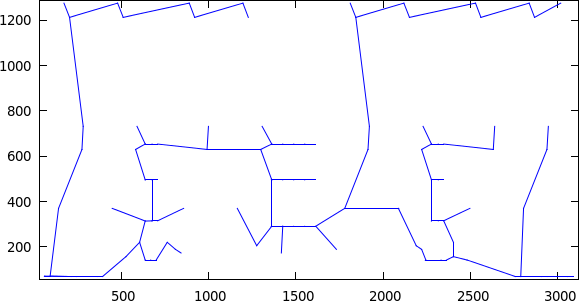
\includegraphics[width=0.48\textwidth]{images/1treelin105}
    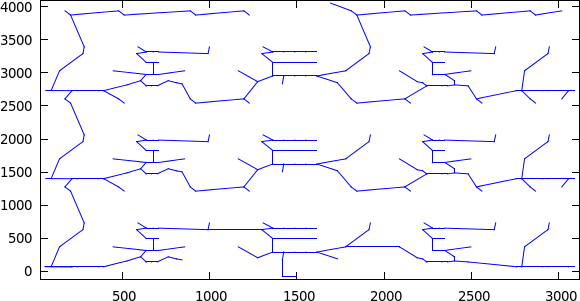
\includegraphics[width=0.48\textwidth]{images/1treelin318}
    \caption{1-albero per \texttt{lin105} e \texttt{lin318}.}
    \label{fig:onetree}
  \end{center}
\end{figure}

\section{Rilassamento Lagrangiano} 
Riprendendo le considerazioni precedenti, possiamo dire che l'eliminazione dei vincoli di grado permette da una parte di poter disporre in modo molto efficiente di un lower bound alla soluzione ottima, dall'altra rende tuttavia il valore ottenuto poco significativo perchè molto al di sotto della soluzione ottima. Il rilassamento lagrangiano che ora andremo a considerare, tenta di migliorare il bound cercando di ristabilire i corretti vincoli di grado per ogni vertice.
Il \emph{rilassamento lagrangiano} è una tecnica di rilassamento per problemi di ottimizzazione: l'idea di base è quella di eliminare dal problema originale una parte di vincoli, possibilmente proprio quei vincoli che rendono difficile la risoluzione del problema, inserendoli nella funzione obiettivo per tenerne in qualche modo conto durante la risoluzione.

Nel nostro caso, andremo a considerare il rilassamento lagrangiano che si ottiene eliminando dal modello i vincoli di grado sui vertici $\{2, ..., n\}$, per inserirli nella funzione obiettivo come somma pesata secondo opportuni coefficienti o \emph{moltiplicatori lagrangiani} $\pi_2, ..., \pi_n$. È da notare come i moltiplicatori non siano vincolati in segno, dal momento che i vincoli eliminati sono in forma di equazioni. Il problema rilassato è detto \emph{problema lagrangiano}, e può essere risolto efficientemente: un algoritmo per la costruzione di un 1-albero minimo basato ad esempio sull'algoritmo di Prim per il calcolo di un MST ci porge una facile soluzione.
\begin{align}
  \min \ \sum_{e \in E} & c_ex_e - \sum^n_{i = 2}\pi_i(\sum_{e \in \delta(v)}x_e - 2) \label{eqn:rxof}\\
  \sum_{e \in \delta(1)} & x_e = 2 \label{eqn:rxdegconst}\\
  \sum_{e \in E(S)}  & x_e \leq |S| - 1 \quad\forall\: S \subset V \setminus \{ 1 \},\; | S | \geq 2 \label{eqn:secs}\\
  \sum_{e \in E \setminus \delta(1)} & x_e = n - 2 \label{eqn:rxnumedg}\\
  & x_e \in \{0,1\}  \quad \forall\: e \in E. \label{eqn:rxinteger}
\end{align}
Come si può osservare, sono stati rilassati i vincoli 1.1 per $v \in V \setminus \{ 1 \}$, mentre \ref{eqn:rxnumedg}, \ref{eqn:secs}, \ref{eqn:rxnumedg}, \ref{eqn:rxinteger} corrispondono al modello matematico di un 1-albero: le soluzioni ammissibili del problema lagrangiano sono tutti e solo gli 1-alberi del grafo. La funzione:
\begin{equation}
L(\pi) = \min \left\{ \sum_{e \in E} c_ex_e - \sum^n_{i = 2}\pi_i(\sum_{e \in \delta(v)}x_e - 2) : x \in X \right\}
\end{equation}
dove $X$ è l'insieme dei vettori di incidenza degli 1-alberi sul grafo, è detta 	\emph{funzione lagrangiana}.

Il valore $L(\pi)$ costituisce un lower-bound al costo di una soluzione ottima del problema originario (che ricordiamo essere un problema di minimizzazione), per qualsiasi vettore di moltiplicatori $\pi$. Per ottenere un buon lower bound si può quindi cercare di massimizzare il valore di $L(\pi)$ al variare di $\pi$, ovvero cercare di risolvere il \emph{problema lagrangiano duale}.

\section{Metodo del Subgradiente} 
La funzione lagrangiana $L:\pi \longrightarrow L(\pi)$ è una funzione continua, lineare a tratti e concava. La ricerca del massimo è complicata dal fatto che la funzione non è differenziabile in ogni suo punto: uno degli approcci più seguiti è quello che utilizza il \emph{metodo del subgradiente}, che tenta di trovare una soluzione generando iterativamente una successione di vettori $\pi^0, \pi^1, ..., \pi^k$ convergente all'ottimo, secondo una regola generale del tipo:
\begin{equation}
\pi^{k+1}_i = \pi^k_i + t^k s^k_i \text{\: \: \: } i = 1, ..., n \label{eqn:hkupdate}
\end{equation}
dove $s^k$ è un subgradiente di $L$ in $\pi^k$, mentre $t^k$ è l'ampiezza dello spostamento che l'algoritmo compie nella direzione determinata dal subgradiente. Con riferimento al modello matematico del problema originario, si dimostra che $(Ax^k - 2)$ è un subgradiente di $L(\pi^k)$ in $\pi^k$, dove $A$ è la matrice dei vincoli di grado. In altre parole, la componente $i$-esima del vettore subradiente all'iterazione $k$-esima è dato da $s^k_i = d_i - 2$, dove $d_i$ è il numero di lati incidenti sul vertice $i$ dell'1-albero calcolato in quell'iterazione. 
La scelta del passo, che peraltro condiziona pesantemente la rapidità con cui l'algoritmo si avvicina all'ottimo, risulta al contrario meno chiara. Si dimostra tuttavia in \citet*{held1970traveling} che la scelta di un passo che verifica le condizioni:
\begin{align}
\lim_{k \to \infty} t^k &= 0 \label{eqn:hksuffcond1} \\
\sum^{\infty}_{k = 0} t^k &= +\infty \label{eqn:hksuffcond2}
\end{align}
garantisce la convergenza all'ottimo della successione di punti $\pi^k$ calcolati ad ogni iterazione seguendo la direzione $s^k / \parallel s^k \parallel$. La formula proposta da Held e Karp è la seguente:
\begin{equation}
t^k = \alpha^k \frac{UB - L(\pi^k)}{{\parallel s^k \parallel}^2} \label{eqn:hkstep}
\end{equation}
dove $UB$ è un upper bound, possibilmente di buona qualità, al valore della soluzione ottima del problema originario, mentre $\alpha^k$ è uno scalare inizialmente posto uguale a 2, e fatto decrescere al procedere dell'algoritmo.

Nonostante \ref{eqn:hkstep} rispetti le due condizioni sufficienti per la convergenza \ref{eqn:hksuffcond1} e \ref{eqn:hksuffcond2}, nessuna garanzia è data circa la velocità con cui l'algoritmo si avvicina all'ottimo. Un metodo alternativo per aggiornare il passo e portare più rapidamente l'algoritmo in prossimità dell'ottimo è invece quello proposto da Volgenant e Jonker. \citet*{volgenant1982branch} impongono che la successione di passi $t^k$ debba rispettare il vincolo imposto da una equazione alle differenze del secondo ordine del tipo: 
\begin{equation}
t^{k+1} - 2 t^k + t^{k-1} = costante
\end{equation}
unitamente alle condizioni $t^1 - t^2 = 3(t^{M-1} - t^M)$ e $t^M = 0$, dove $M$ è il massimo numero di iterazioni che si intende far compiere all'algoritmo. La regola di aggiornamento del passo che ne consegue è la seguente:
\begin{equation}
t^k = t^1 \frac{k^2 - 3 (M - 1) k + M (2 M - 3)}{2 (M - 1) (M - 2)} \label{eqn:vjstep}
\end{equation}
Come si può notare, la regola è completamente specificata una volta scelto il numero massimo di iterazioni $M$ e l'ampiezza del primo passo $t^1$, mentre non richiede, contrariamente alla regola di Held e Karp, la conoscenza di un buon upper bound per poter essere utilizzata. Come vedremo, sarà proprio questa caratteristica a permetterci di sfruttare il metodo del subgradiente anche nei nodi interni dell'albero di ricerca del branch-and-bound. Sempre in \citep{volgenant1982branch}, viene suggerita la seguente formula per il calcolo della nuova posizione ad ogni iterazione:
\begin{align}
\pi^{k+1}_i = \pi^k_i + 0.6 \: t^k (d^k_i - 2) + 0.4 \: t^k (d^{k-1}_i - 2)  \text{\: \: \:} i = 1, ..., n  \label{eqn:vjupdate}
\end{align}
dove l'inserimento del termine $t^k (d^{k-1}_i - 2)$, ovvero della componente $i$-esima del subgradiente all'iterazione precedente, ha lo scopo di smorzare le oscillazioni nella direzione di spostamento che incorrono quando l'algoritmo si trova a confine di due o più zone in cui la funzione lagrangiana assume differenti gradienti (fenomeno detto zig-zagging). 

Una nostra prima implementazione cerca di risolvere il problema lagrangiano duale utilizzando il metodo del subgradiente e le regole \ref{eqn:hkstep} e \ref{eqn:hkupdate} per l'aggiornamento del passo e della posizione. Una seconda implementazione segue invece le regole \ref{eqn:vjstep} e \ref{eqn:vjupdate}. In entrambi i casi, la costruzione dell'1-albero viene effettuata sfruttando l'algoritmo di Prim per la costruzione di alberi di supporto minimo. Proponiamo infine una terza soluzione, in cui l'albero di supporto minimo viene calcolato con l'algoritmo di Kruskal, mentre l'avanzamento dell'algoritmo del subgradiente è regolato da \ref{eqn:vjstep} e \ref{eqn:vjupdate}. Chiameremo di seguito le tre soluzioni rispettivamente come PHK (Prim-Held-Karp), PVJ (Prim-Volgenant-Jonker) e KVJ (Kruskal-Volgenant-Jonker).

Le immagini \ref{fig:phk1}, \ref{fig:pvj1} e \ref{fig:kvj1} mostrano l'andamento dell'aggiornamento del lower bound, vale a dire come varia il bound quando viene individuata una soluzione migliorante. Le immagini \ref{fig:phk2}, \ref{fig:pvj2} e \ref{fig:kvj2}, invece, mostrano il valore del bound ad ogni iterazione del subgradiente.

\begin{figure}
  \begin{center}
    \includegraphics[width=0.48\textwidth]{images/prlagrangehk1gr137}
    \includegraphics[width=0.48\textwidth]{images/prlagrangehk3fl417}
    \caption{Miglioramento del lower bound con PHK per \texttt{gr137} e \texttt{fl417}.}
    \label{fig:phk1}
      
    \includegraphics[width=0.48\textwidth]{images/prvjgr1371}
    \includegraphics[width=0.48\textwidth]{images/prvjfl4171}
    \caption{Miglioramento del lower bound con PVJ per \texttt{gr137} e \texttt{fl417}.}
    \label{fig:pvj1}

    \includegraphics[width=0.48\textwidth]{images/krvjgr1371}
    \includegraphics[width=0.48\textwidth]{images/krvjfl4171}
    \caption{Miglioramento del lower bound con KVJ per \texttt{gr137} e \texttt{fl417}.}
    \label{fig:kvj1}
  \end{center}
\end{figure}

\begin{figure}
  \begin{center}
    \includegraphics[width=0.48\textwidth]{images/prlagrangehk3gr137}
    \includegraphics[width=0.48\textwidth]{images/prlagrangehk2fl417}
    \caption{Andamento complessivo del lower bound con PHK per \texttt{gr137} e \texttt{fl417}.}
    \label{fig:phk2}
      
    \includegraphics[width=0.48\textwidth]{images/prvjgr1372}
    \includegraphics[width=0.48\textwidth]{images/prvjfl41721}
    \caption{Andamento complessivo del lower bound con PVJ per \texttt{gr137} e \texttt{fl417}.}
    \label{fig:pvj2}

    \includegraphics[width=0.48\textwidth]{images/krvjgr1372}
    \includegraphics[width=0.48\textwidth]{images/krvjfl41721}
    \caption{Andamento complessivo del lower bound con KVJ per \texttt{gr137} e \texttt{fl417}.}
    \label{fig:kvj2}
  \end{center}
\end{figure}

\subsection{Subgradiente PHK}
Il primo metodo è quello proposto inizialmente in \citep{held1970traveling}. Come anticipato, in questa implementazione la costruzione di un 1-albero ad ogni iterazione segue l'algoritmo di Prim. Una particolare attenzione è stata posta nell'adattare l'algoritmo per renderlo compatibile con la nostra decisione di trattare in modo esplicito i vincoli sui lati del grafo, senza dover ricorrere ad artifici come l'assegnazione di un costo molto grande o molto piccolo rispettivamente per vietare o forzare un lato. Questa scelta ha forse complicato alcune porzioni di codice, ma ci ha permesso di procedere senza dover prestare attenzione ad eventuali comportamenti imprevisti dovuti a combinazioni di costi particolarmente elevati. 

La messa a punto di parametri quali il coefficiente $\alpha^k$ o il numero massimo di iterazioni si è rivelata particolarmente ostica, mostrando perlomeno inizialmente risultati poco soddisfacenti, oppure molto buoni ma solo su ristretti gruppi di istanze, su cui i parametri risultavano evidentemente sovradattati. Ricalcando alcune idee utilizzate in \citep{volgenant1982branch}, è stato deciso di utilizzare un numero massimo $M$ di iterazioni proporzionale a $n^2$, la dimensione dell'istanza; $\alpha$ viene invece dimezzato ogni qual volta viene superato un certo numero $h$ di iterazioni consecutive senza conseguire alcun miglioramento nella valutazione del massimo della funzione lagrangiana. Il valore di $h$ è stato calcolato come segue: se $h$ fosse il tempo medio di dimezzamento di $\alpha$, ci sarebbero all'incirca $M/h$ dimezzamenti nel corso dell'algoritmo; imponendo $\alpha_u = 0.001$ all'ultimo aggiornamento $u = M/h$, si trova $h = M / (\log_2{\alpha_1} - \log_2{0.001})$, dove $\alpha_1 = 2$ è il valore assunto inizialmente.

\begin{figure}
  \begin{center}
    \includegraphics[width=0.48\textwidth]{images/prlagrangehk4gr137}
    \includegraphics[width=0.48\textwidth]{images/prlagrangehk5gr137}
    \caption{Dettagli dell'aggiornamento del bound per \texttt{gr137}.}
    \label{fig:phkdettagli}
  \end{center}
\end{figure}

In figura \ref{fig:phkdettagli} mostriamo dei dettagli dell'aggiornamento con PHK per \texttt{gr137} come riportato in figura \ref{fig:phk2}.

\subsection{Subgradiente PVJ}
In questa implementazione il passo e la direzione sono aggiornati seguendo le regole \ref{eqn:vjstep} e \ref{eqn:vjupdate}, mentre il numero massimo di iterazioni è pari a $n^2 / 50 + n + 16$, come suggerito in \citep{volgenant1982branch}. Il passo di base $t^1$ che compare in \ref{eqn:vjstep} è posto inizialmente pari a $L(\pi^1) / n$, ed è successivamente aggiornato ogni qual volta l'algoritmo migliora il valore della funzione lagrangiana \footnote{Il valore scelto in [2] per $t^1$ è $L(\pi^1) * 0.01$, dove il fattore $0.01$ è stato presumibilmente scelto in rapporto alla dimensione delle istanze risolte, che all'epoca difficilmente superava le $100$ città.}. Come si vedrà anche più avanti, esiste per questa implementazione la possibilità di essere eseguita in una modalità leggermente differente, ottimizzata rispetto al caso in cui ci si trovi ad operare in un nodo interno dell'albero di ricerca del branch-and-bound. In questo caso, il numero massimo di iterazioni viene notevolmente ridotto, mentre il valore dello step di base viene calcolato in base al valore dei moltiplicatori corrispondenti alla migliore soluzione trovata dall'algoritmo quando eseguito nel nodo radice dell'albero di ricerca. Sempre con riferimento ad un contesto di branch-and-bound, un accorgimento particolarmente efficace è inoltre quello di interrompere l'esecuzione e uscire dal loop principale di iterazione non appena viene trovato un valore della funzione lagrangiana superiore all'incumbent.

\begin{figure}
  \begin{center}
    \includegraphics[width=0.48\textwidth]{images/prvjfl41722}
    \caption{Dettaglio dell'aggiornamento del bound per \texttt{fl417}.}
    \label{fig:pvjdettagli}
  \end{center}
\end{figure}

Riportiamo in figura \ref{fig:pvjdettagli} il dettaglio delle ultime iterazioni di PVJ su \texttt{fl417}.

\subsection{Subgradiente KVJ}
L'implementazione che ora descriveremo, a differenza delle precedenti, utilizza l'algoritmo di Kruskal per il calcolo di un albero ricoprente minimo. La complessità computazionale dell'algoritmo di Prim, quadratica nel numero di nodi dell'istanza, non permette di sfruttare appieno eventuali riduzioni del problema iniziale in termini di numero di lati. L'aggiunta di vincoli iniziali sui lati non è certo trasparente ad un branch-and-bound in cui l'1-albero viene calcolato utilizzando l'algoritmo di Prim, visto che il fissaggio dei lati riduce le possibili strade nell'albero di ricerca; ciò che però si vorrebbe ottenere è anche uno speed-up all'interno di ogni singolo nodo, come conseguenza diretta di una effettiva diminuzione della dimensione dell'istanza. Come indicato dai test effettuati, i vantaggi di questo approccio riescono a bilanciare e superare alcune evidenti limitazioni dell'algoritmo di Kruskal, a partire proprio dalla sfavorevole complessità computazionale nel caso di grafi completi o più in generale densi.
\paragraph*{}
La rapidità dell'algoritmo è principalmente ostacolata dalla difficoltà di effettuare efficientemente le due seguenti operazioni:
\begin{enumerate}[noitemsep]
\item ordinare i lati del grafo in base al loro costo
\item verificare che l'aggiunta di un lato alla soluzione sia consistente con i vincoli di aciclicità
\end{enumerate}
Per quanto riguarda il punto $2$, abbiamo affrontato il problema realizzando una struttura dati di tipo \emph{union-find}, utilizzata ogni qualvolta l'algoritmo cerca di aggiungere un lato $(i, j)$ alla soluzione. Le procedure $find(i)$ e $find(j)$ vengono chiamate per verificare se $i$ e $j$ appartengono o meno alla stessa componente connessa: in caso positivo il lato viene scartato dalla soluzione, altrimenti viene aggiunto e la procedura $union(i, j)$ aggiorna la struttura per tenere traccia della nuova componente connessa formatasi. Dal momento che la procedura $union$ viene utilizzata al più  $n-2$ volte, mentre $find$ è utilizzato un numero di volte che è circa pari al numero di lati del grafo, sì è deciso di progettare la struttura in modo tale che $find$ avesse complessità $O(1)$. Per rendere inoltre il costo complessivo delle $n-2$ operazioni $union$ dell'ordine $O(n\log(n))$, l'unione di due componenti separate avviene aggiornando gli elementi della componente con minor numero di elementi. Naturalmente, una volta aggiunti gli $n-2$ lati corrispondenti alla porzione mst dell'1-albero, non è necessario continuare a processare i rimanenti.

Per quanto riguarda invece la problematica evidenziata al punto $1$, una soluzione è stata tentata affidando l'ordinamento dei lati alla funzione \emph{qsort} della libreria standard di C. Come ci si poteva aspettare, la complessità computazionale di quicksort non ha permesso di ottenere significativi miglioramenti rispetto alle soluzioni Prim-based, anche in caso di grafi notevolmente ridotti. È stata invece scartata fin da subito la possibilità di un ordinamento di tipo merge-sort, non essendo un algoritmo in-place. Si è deciso quindi di sfruttare l'interezza dei costi (nel caso di istanze TSPLIB) per migrare verso l'utilizzo di algoritmi di ordinamento non comparativi, in particolare counting-sort. I lati possono essere facilmente ordinati considerando come chiave il loro stesso costo, e la complessità computazionale di questa operazione è data da:
\begin{equation}
T_{cs} = 2 N + K
\end{equation}
dove $N$ è il numero di lati da ordinare e $K$ e il numero di possibili chiavi. Se $c_{min}$ e $c_{max}$ sono rispettivamente il costo minimo e il costo massimo tra i costi dei lati da ordinare, il numero di chiavi è dato da $K = c_{max} - c_{min} + 1$. Sebbene si possa osservare che per la maggior parte delle istanze TSPLIB il range di possibili costi non supera il numero di lati del grafo completo, per alcune istanze la differenza di costo tra i lati da ordinare potrebbe rallentare notevolmente l'ordinamento. Bisogna inoltre ricordare che i costi dei lati durante le varie iterazioni del subgradiente vengono modificati dai moltiplicatori lagrangiani, e il range dei costi potrebbe aumentare. Infine, il peso di $K$ risulta certamente più rilevante quanto più il numero $N$ di lati da ordinare diminuisce, ovvero proprio nei casi in cui vorremmo trarre beneficio dalla nostra implementazione Kruskal-based. Per aggirare questo problema si è reso necessario implementare un ulteriore algoritmo di ordinamento di tipo radix-sort, da utilizzare quando il numero di chiavi supera di una certa soglia il numero di lati da ordinare. La complessità computazionale di radix-sort è data da:
\begin{equation}
T_{rx} = 2 N d  + d b
\end{equation}
dove $d = \log_b{K}$. Scegliendo come base $b = N$ si ottiene una complessità pari a $3 N d$, dove $d = \log_N{K}$. 

Descriviamo brevemente le principali fasi attraversate ad ogni iterazione.
\begin{enumerate}[noitemsep]
\item Viene costruito un 1-albero a partire da una lista di lati ordinati composta all'iterazione precedente. 
\item Vengono calcolati i nuovi moltiplicatori: dal momento che intendiamo trattare solamente costi interi, i moltiplicatori vengno arrotondati all'intero più vicino prima di essere utilizzati per aggiornare i costi dei lati del problema lagrangiano. Il prezzo da pagare sarà una generale peggioramento nella qualità del lower bound ritornato. 
\item Vengono aggiornati i costi dei lati a partire dai moltiplicatori correnti.
\item I lati vengono ordinati in base al loro costo.
\end{enumerate}

L'algoritmo può essere reso ancora più efficiente se si considera che nel corso della sua evoluzione, tende a modificare con sempre minor frequenza i valori assunti dai moltiplicatori; molti di essi si assestano su pesi che manterranno invariati fino alla fine dell'esecuzione. Come conseguenza, il numero di lati i cui costi vengono modificati tende generalmente a diminuire al crescere del numero di iterazioni (si vedano le figure in \ref{fig:kvj3}). L'idea è quella di estrarre dalla lista globale dei lati $L$, ereditata già ordinata dall'iterazione precedente, quei lati i cui costi sono stati modificati nell'iterazione corrente, formando una lista $L_{ch}$ di lati modificati. I lati rimanenti formeranno invece una lista $L_{nch}$ già ordinata. Ci possiamo quindi limitare l'applicazione degli algoritmi di ordinamento, il fattore computazionalmente più pesante di tutta la procedura, alla sola lista $L_{ch}$. Una nuova lista di lati ordinata utilizzabile dall'algoritmo di Kruskal all'iterazione successiva viene infine creata in tempo lineare effettuando un semplice merge tra $L_{ch}$ e $L_{nch}$. 
Gli algoritmi di ordinamento utilizzati sono, come già detto, counting-sort e radix-sort, unitamente a quicksort per gestire eventuali fasi finali del subgradiente, in cui il numero di lati modificati diminuisce a tal punto rispetto al numero di chiavi utilizzate da rendere poco conveniente l'utilizzo dello stesso radix-sort rispetto a quicksort.

\begin{figure}
  \begin{center}
    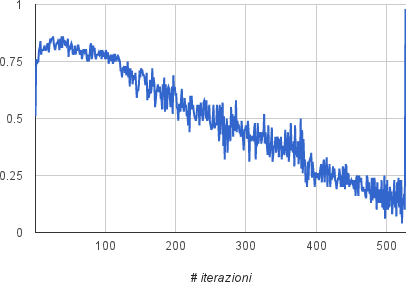
\includegraphics[width=0.7\textwidth]{images/gr137chgedges}
    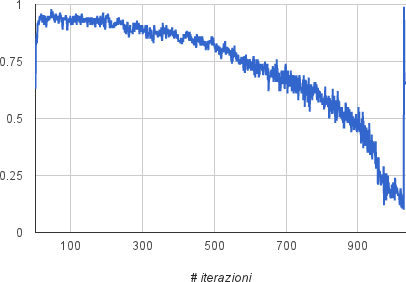
\includegraphics[width=0.7\textwidth]{images/gr202chgedges}
    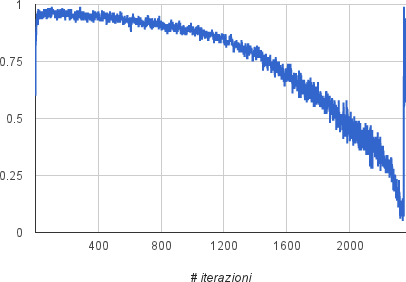
\includegraphics[width=0.7\textwidth]{images/lin318chgedges}
    \caption{Andamento del numero di lati con costi modificati (frazione sul totale) per \texttt{gr137}, \texttt{gr202}, \texttt{lin318}.}
    \label{fig:kvj3}
  \end{center}
\end{figure}

\section{Branch-and-Bound}
Nella sua implementazione di base il branch-and-bound (\citet*{land1960automatic}) è una ricerca in profondità in cui ad ogni nodo viene selezionata una variabile della soluzione frazionaria, e relativamente ad essa viene effettuata una scelta, che porta alla generazione di due sottoalberi: in uno la variabile viene arrotondata all'intero inferiore, nell'altro viene invece arrotondata all'intero superiore. Questa operazione è detta \emph{branching}. In generale, ad ogni nodo viene effettuata una decisione tale da partizionare il sottospazio di ricerca in sottoalberi mutuamente disgiunti, garantendo in questo modo sia la completezza della ricerca che l'unicità del cammino per raggiungere la soluzione. Ad ogni nodo, la soluzione generata viene inoltre confrontata con i bound alla soluzione ottima disponibili a quel punto della ricerca: nel caso si tratti di un problema di minimizzazione, se il costo è superiore o uguale all'upper bound (detto anche \emph{incumbent}), il ramo di branching può essere rimosso e il sottoalbero associato scartato, dal momento che non potrà contenere una soluzione ammissibile di costo minore. Infine, sempre nel caso di problemi di minimizzazione, se ad un nodo viene generata una soluzione ammissibile di costo inferiore all'incumbent, quest'utlimo verrà aggiornato al costo della nuova soluzione.
\paragraph*{}
Discutiamo di seguito alcuni aspetti della nostra implementazione, che fa uso degli algoritmi precedentemente presentati. Tutte le versioni proposte fanno uso della regola di branching proposta da Volgenant e Jonker in \citep{volgenant1982branch}, e attraversano i rami preferendo nell'ordine i caso in cui i due lati selezionati $e_1$ ed $e_2$ vengono entrambi forzati, il caso in cui $e_1$ viene forzato ed $e_2$ viene vietato, infine il caso in cui $e_1$ viene vietato. 
\subsection{B \& B Prim-based}
Una prima versione che abbiamo implementato utilizza PVJ per la computazione di un buon lower-bound ad ogni nodo. Nonostante PVJ riesca a garantire bound di qualità migliore rispetto a KVJ, la complessità quadratica nel numero dei nodi non permette incrementi nella velocità di esecuzione a seguito di riduzioni. Di questa versione, come della successiva, sono state provate alcune varianti, modificando alcuni parametri o inserendo o meno metodi di riduzione e propagazione.

\subsection{B \& B Kruskal-based}
Una seconda versione utilizza invece KVJ, per sfruttare al massimo le riduzioni applicate al grafo di partenza e l'imposizione di vincoli durante la discesa nell'albero di ricerca. In questa implementazione, viene mantenuta una lista concatenata di lati non vincolati, aggiornata ogni volta prima di passare ad un nodo figlio, e viceversa al ritorno per ripristinare le condizioni inizialmente presenti.
%\paragraph*{}
In entrambe le versioni, generalizzando quanto suggerito in [3], ogni nodo eredita i moltiplicatori lagrangiani associati alla migliore soluzione trovata dal nodo padre: tali moltiplicatori vengono utilizzati come punto di partenza per l'algoritmo del subgradiente, e a partire da essi viene calcolata l'ampiezza dello step iniziale.
\subsection{Riduzione dei lati}\label{sec:riduzionelati}
Per rendere vantaggioso l'utilizzo di KVJ rispetto a PVJ, è necessaria l'applicazione al grafo iniziale di una buona riduzione. La riduzione implementata prevede la costruzione di un 1-albero minimo, il calcolo dei \emph{costi marginali} associati a ciascun lato del grafo, e infine l'eliminazione di quei lati i cui costi ridotti superano una certa soglia, con la garanzia che tali lati certamente non appartengono alla soluzione ottima. L'osservazione che sta alla base del meccanismo di riduzione utilizzato, è la seguente: dato un 1-albero minimo $T$ per il grafo $G$, un lato $e$ può essere eliminato se una sua forzatura costringe l'1-albero minimo ad assumere un valore maggiore rispetto ad un upper bound alla soluzione ottima. Se $T(e)$ è l'1-albero minimo ottenuto forzando il lato $e$ in $T$, si definisce come costo marginale di $e$ il valore $\bar{c_e} = c(T(e)) - c(T)$, e il lato può essere rimosso senza escludere la soluzione ottima dalla regione ammissibile se:
\begin{equation}
c(T(G) + \bar{c_e} > UB
\end{equation}
La correttezza di tale procedura è garantita (\citep{benchimol2010improving,benchimol2012improved}) anche nel caso in cui $T(G)$ sia un 1-albero ottenuto da un rilassamento lagrangiano del tipo proposto da Held e Karp. Nel nostro caso, una riduzione di questo tipo è applicata inizialmente, utilizzando il migliore 1-albero calcolato da PHK. Abbiamo poi esplorato la possibilità di utilizzare la stessa riduzione anche all'interno dell'albero di ricerca, prestando attenzione a ristabilire i lati rimossi prima di risalire ad un livello superiore. Per evitare di appesantire troppo la computazione, la riduzione viene eseguita in un determinato nodo solamente quando viene rilevato un restringimento del gap tra lower e upper bound rispetto al gap registrato nel nodo padre.
\subsection{Propagazione dei vincoli}
Un'altra tecnica per cercare di ridurre lo spazio di ricerca è quella di aggiungere tutti quei vincoli che possono essere derivati a partire dalla presente disposizione dei vincoli sul grafo, oppure verificare la consistenza dei vincoli che dovranno essere aggiunti per scartare eventuali branch non ammissibili prima di iniziare la computazione nei nodi figli. Una prima osservazione per procedere in tal senso è la seguente: se ci sono due lati forzati incidenti in un vertice, è possibile vietare tutti i rimanenti lati incidenti su quello stesso vertice, dal momento che i vincoli di grado impongono che vi siano esattamente due lati incidenti in ogni vertice della soluzione. Analogamente, se ci sono $n-3$ lati vietati incidenti in un vertice, è possibile forzare i rimanenti due lati. 

L'imposizione di vincoli ai lati incidenti in un nodo con due lati forzati o $n-3$ lati vietati modifica il numero di lati forzati e vietati incidenti nei nodi vicini, rendendo eventualmente possibile applicare su di essi lo stesso procedimento qualora le condizioni siano verificate. L'idea è quindi di procedere ricorsivamente propagando l'imposizione di vincoli ai nodi vicini. A partire da queste considerazioni abbiamo implementato una procedura che, prima di attraversare un nuovo ramo dell'albero di ricerca, impone e cerca di propagare i vincoli associati a quel branch, verificando infine la presenza di eventuali inconsistenze. Prima di passare al branch successivo o risalire l'albero di ricerca, viene effettuato un rollback per ristabilire i vincoli preesistenti.

\section{Risultati computazionali}
\subsection{Subgradiente lagrangiano}
\afterpage{%
    \clearpage% Flush earlier floats (otherwise order might not be correct)
    \thispagestyle{empty}% empty page style (?)
\begin{scriptsize}
\begin{center}
    \begin{longtabu} to \linewidth {c|S[table-format=3.2]S[table-format=4.2]|S[table-format=3.2]S[table-format=4.2]|S[table-format=3.2]S[table-format=4.2]|S[table-format=6.2]}
    \toprule
    \multicolumn{1}{c}{} & \multicolumn{2}{c}{PHK} & \multicolumn{2}{c}{PVJ} & \multicolumn{2}{c}{KVJ} & \multicolumn{1}{c}{}  \\
    Istanza & $z$ &  T [s] & $z$ &  T [s] & $z$ &  T [s]  & $z^*$ \\
    \midrule
    \endhead
a280 &  99.50 & 33.54 &  99.49 & 1.65 &  98.94 & 1.61  &  2566.00 \\
ahk48 &  99.83 & 0.04 &  99.81 & 0.00 &   99.81 & 0.00  &  11441.31 \\
ali535 &  99.47 & 218.44 &  99.40 & 31.36 &   99.37 & 78.53  &  201236.24 \\
att48 &  99.77 & 1.30 &  99.69 & 0.01 &   99.70 & 0.00  &  9029.00 \\
att532 &  95.58 & 193.52 &  95.57 & 25.09 &   95.44 & 66.58  &  27419.14 \\
berlin52 &  \textbf{100.00} & 0.05 &  \textbf{100.00} & 0.00 &  \textbf{100.00} & 0.01  &  7542.00 \\
bier127 &  99.28 & 1.61 &  99.27 & 0.10 &   99.27 & 0.16  &  95331.00 \\
ch130 &  99.44 & 1.93 &  99.40 & 0.12 &   99.27 & 0.10  &  6075.50 \\
ch150 &  99.42 & 3.56 &  99.37 & 0.19 &  99.25 & 0.17  &  6490.12 \\
d198 &  99.57 & 8.45 &  99.55 & 0.44 &   99.46 & 0.65  &  15712.00 \\
d493 &  99.50 & 153.44 &  99.49 & 16.53 &  99.34 & 40.99  &  34828.49 \\
d657 &  99.07 & 427.04 &  99.05 & 78.32 &  99.00 & 187.93  &  48455.17 \\
eil101 &  99.76 & 0.70 &  99.69 & 0.04 &  99.57 & 0.03  &  627.50 \\
eil51 &  99.18 & 0.05 &  99.12 & 0.00 &  99.03 & 0.01  &  422.50 \\
eil76 &  99.74 & 0.24 &  99.79 & 0.02 &   99.73 & 0.01  &  536.90 \\
fl417 &  99.40 & 128.11 &  99.39 & 10.55 &  99.28 & 26.14  &  11789.50 \\
fri26 &  \textbf{100.00} & 0.00 &  \textbf{100.00} & 0.00 &  99.94 & 0.01 &  937.00 \\
gil262 &  99.01 & 33.01 &  99.00 & 1.49 &   98.60 & 1.31  &  2354.50 \\
gr137 &  98.95 & 1.91 &  98.93 & 0.11 & 98.93 & 0.19 &  69120.25 \\
gr17 &  \textbf{100.00} & 0.00 &  95.70 & 0.00 &  95.37 & 0.00  &  2085.00 \\
gr202 &  99.74 & 9.50 &  99.73 & 0.47 &  99.73 & 0.75 &  40055.00 \\
gr21 &  \textbf{100.00} & 0.00 &  \textbf{100.00} & 0.00 &  \textbf{100.00} & 0.00 &  2707.00 \\
gr229 &  99.05 & 14.61 &  99.03 & 0.74 &  99.03 & 1.51 &   133317.02 \\
gr24 &  \textbf{100.00} & 0.00 &  99.96 & 0.00 &  99.76 & 0.00 &  1271.98 \\
gr48 &  98.28 & 0.05 &  98.25 & 0.00 &  98.19 & 0.01 &  4959.00 \\
gr666 &  99.37 & 349.28 &  99.36 & 72.04 &  99.35 & 200.54  &  292493.34 \\
gr96 &  98.84 & 0.48 &  98.84 & 0.03 &  98.83 & 0.04 &  54570.50 \\
hk48 &  99.83 & 0.04 &  99.81 & 0.00 &  99.81 & 0.00  &  11441.31 \\
kroA100 &  98.38 & 0.75 &  98.37 & 0.05 &  98.35 & 0.05 &  20936.50 \\
kroA150 &  99.15 & 3.53 &  99.14 & 0.19 &  99.11 & 0.26  &  26299.00 \\
kroA200 &  98.97 & 11.14 &  98.94 & 0.54 &  98.93 & 0.58  &  29065.00 \\
kroB100 &  98.61 & 0.73 &  98.61 & 0.05 &   98.60 & 0.06 &    21834.00 \\
kroB150 &  98.48 & 3.60 &  98.47 & 0.19 &  98.44 & 0.26 &    25732.50 \\
kroB200 &  99.08 & 11.01 &  99.07 & 0.54 &  99.05 & 0.55 &   29165.00 \\
kroC100 &  98.67 & 0.72 &  98.66 & 0.05 &  98.65 & 0.05 &    20472.50 \\
kroD100 &  99.28 & 0.73 &  99.27 & 0.05 &  99.26 & 0.05 &   21141.50 \\
kroE100 &  98.78 & 0.73 &  98.78 & 0.05 &   98.78 & 0.05 &   21799.50 \\
lin105 &  99.94 & 0.68 &  99.94 & 0.04 &  99.94 & 0.06 &  14370.38 \\
lin318 &  99.67 & 57.15 &  99.66 & 2.73 &  99.65 & 5.52 & 41888.75 \\
p654 &  96.87 & 318.87 &  99.83 & 66.61 &  99.46 & 137.72 &   34582.78 \\
pcb442 &  99.45 & 150.48 &  99.41 & 11.96 &  99.34 & 25.31 &  50499.49 \\
pr107 &  87.25 & 0.72 &  81.96 & 0.04 &  81.23 & 0.09 &  44302.48 \\
pr124 &  98.37 & 1.31 &  98.36 & 0.07 &  98.36 & 0.09 &  58067.50 \\
pr136 &  99.13 & 2.07 &  99.09 & 0.12 &  99.07 & 0.20 &  95934.49 \\
pr144 &  99.41 & 2.40 &  99.40 & 0.16 &  99.40 & 0.21 &  58189.25 \\
pr152 &  99.36 & 3.03 &  98.24 & 0.16 &  98.27 & 0.29 &  73207.57 \\
pr226 &  99.66 & 14.16 &  99.65 & 0.72 &    99.64 & 1.33 & 80092.00 \\
pr264 &  99.73 & 26.44 &  99.77 & 1.29 &  99.76 & 2.25 &  49019.86 \\
pr299 &  98.32 & 42.15 &  98.31 & 2.06 &    98.29 & 2.93 &  47380.00 \\
pr439 &  98.80 & 135.56 &  98.78 & 9.67 &   98.77 & 31.25 &  92443.00 \\
pr76 &  97.17 & 0.20 &  97.18 & 0.02 &  97.18 & 0.02 &  90111.00 \\
rat195 &  98.98 & 7.69 &  98.81 & 0.40 &  98.37 & 0.39  &  2299.25 \\
rat575 &  99.28 & 262.04 &  99.27 & 40.17 &  98.68 & 75.13  &  6723.99 \\
rat783 &  99.62 & 667.19 &  99.62 & 185.33 & 99.00 & 380.34 &  8772.74 \\
rat783 &  99.62 & 667.19 &  99.62 & 185.33 &  99.00 & 380.34 &  8772.74 \\
rat99 &  99.59 & 0.54 &  99.57 & 0.03 &  99.25 & 0.04 &   1206.00 \\
rd100 &  99.87 & 0.72 &  99.81 & 0.04 &  99.76 & 0.04 &   7899.33 \\
rd400 &  99.19 & 109.70 &  99.18 & 7.41 &  99.06 & 10.78 &   15157.00 \\
st70 &  99.41 & 0.17 &  99.37 & 0.01 &  99.06 & 0.02 &   671.00 \\
swiss42 &  99.92 & 0.01 &  99.89 & 0.00 &  99.76 & 0.01 &  1272.00 \\
ts225 &  91.28 & 13.96 &  91.27 & 0.70 &  91.26 & 1.04 &   115605.00 \\
tsp225 &  98.96 & 14.53 &  98.94 & 0.72 &  98.62 & 0.71 &  3878.25 \\
u159 &  99.63 & 3.67 &  99.63 & 0.21 &   99.61 & 0.35 &   41925.00 \\
u574 &  99.48 & 268.70 &  99.47 & 42.42 &  99.42 & 92.58 &  36714.00 \\
u724 &  99.39 & 554.70 &  99.38 & 138.04 & 99.31 & 320.33 &   41652.66 \\
ulysses16 &  \textbf{100.00} & 0.00 &  95.75 & 0.00 &  95.83 & 0.00 &  6859.00 \\
ulysses22 &  \textbf{100.00} & 0.00 &  98.24 & 0.00 &  98.28 & 0.00 &   7013.00 \\
\bottomrule
\label{tab:lagr}
    \end{longtabu}
    \captionof{table}{Confronto dei diversi metodi per il subgradiente lagrangiano.}
    \end{center}
\clearpage
\end{scriptsize}
}

In tabella \ref{tab:lagr} sono riportati i risultati ottenuti con le varie implementazioni del subgradiente lagrangiano. I risultati sono in percentuale rispetto all'ottimo, e i tempi sono espressi in secondi; sono evidenziati in grassetto i bound che corrispondono al costo del tour ottimo, segno che il subgradiente lagrangiano ha risolto l'istanza. Sono riportati, da sinistra a destra, i risultati di PHK, PVJ e KVJ. L'ultima colonna riporta il miglior lower bound ottenuto.

Si nota facilmente come PHK sia la soluzione che consente di ottenere i migliori lower bound sia Prim-Held-Karp, che tuttavia è anche la soluzione che impiega il maggior tempo a convergere. Sia PVJ che KVJ riportano lower bound leggermente inferiori (con PVJ appena inferiore come prestazioni rispetto a PHK, mentre KVJ spesso non arriva a pareggiare la qualità della soluzione ottenuta) che tempi decisamente ridotti (anche sotto questo aspetto la soluzione basata su Prim è migliore di quella basata su Kruskal).

Nei test effettuati in seguito si è scelto di adoperare PHK, in quanto un miglior bound consente un preprocessing più efficace in termini di archi eliminati.

\subsection{Branch-and-bound}
\afterpage{%
    \clearpage% Flush earlier floats (otherwise order might not be correct)
    \thispagestyle{empty}% empty page style (?)
\begin{scriptsize}
\begin{landscape}
    \begin{longtabu} to \linewidth {c|rrS[table-format=6.2]S[table-format=4.2]|rrS[table-format=4.2]|rrS[table-format=4.2]|rrS[table-format=4.2]|rrS[table-format=4.2]}
    \toprule
    \multicolumn{1}{c}{} & \multicolumn{4}{c}{} & \multicolumn{3}{c}{BB-PVJ-1} & \multicolumn{3}{c}{BB-KVJ-1} & \multicolumn{3}{c}{BB-PVJ-2} & \multicolumn{3}{c}{BB-KVJ-2} \\
%    \cmidrule(r){4-5} \cmidrule(r){6-7} \cmidrule(r){8-9}
    Istanza & $z^*$ & UB & LB & AR [\%] & \#L & \#N & T [s] & \#L & \#N & T [s] & \#L & \#N & T [s] & \#L & \#N & T [s]  \\
    \midrule
    \endhead
\label{tab:bbres}
att48	 &   10628 &   10628 &   10604 &   91.76  &    5 &   16 &   0.01  &     3 &    12 &    0.01 &     4 &     8 &    0.02  &     3 &     8 &    0.00 \\
berlin52	 &    7542 &    7542 &    7542 &    96.08  &   1 &    1 &     0.00  &   1 &     1 &    0.00 &     1 &     1 &    0.00  &     1 &     1 &    0.00 \\
bier127	 &  118282 &  118282 &  117431 &   87.59  &   34 &   583267 &    3600.01  &    36 &  3777582 & 3600.01 &    27 & 23466 &  470.43  &    25 & 33809 &   92.54 \\
burma14	 &    3323 &    3323 &    3323 &      84.62  &    1 &   1 &  0.00  &  1 &     1 &    0.00 &     1 &     1 &    0.00  &     1 &     1 &    0.00 \\
ch130	 &    6110 &    6110 &    6076 &      93.56  &  22 &  6771 &      43.14  &    29 & 56854 &   45.80 &    26 &  5361 &  101.07  &    31 & 43425 &   99.47 \\
ch150	 &    6528 &    6528 &    6490 &      94.71  &    17 &   1605 &      16.74  &    23 & 10730 &   12.35 &    19 &   719 &   25.15  &    20 &  6582 &   21.09 \\
dantzig42 	 &     699 &     699 &     697 &     90.48  &   3 &      5 &   0.00  &     4 &     7 &    0.00 &     3 &     5 &    0.01  &     3 &     6 &    0.00 \\
eil101	 &     629 &     629 &     628 &     96  &     5 &       41 &       0.22  &    18 &  1034 &    0.54 &     5 &    28 &    0.43  &    15 &   258 &    0.33 \\
eil51	 &     426 &     426 &     423 &    90.59  &    13 &      265 &       0.16  &    23 &  2560 &    0.36 &    13 &   263 &    0.34  &    14 &   216 &    0.09 \\
eil76	 &     538 &     538 &     537 &   95.09  &    15 &       62 &       0.14  &    14 &   919 &    0.32 &    15 &    62 &    0.35  &     6 &    25 &    0.03 \\
fri26	 &     937 &     937 &     937 &      92  &     1 &        1 &    0.00 &     1 &     1 &    0.00 &     1 &     1 &    0.00  &     1 &     1 &    0.00 \\
gr137	 &   69853 &   69853 &   69104 &   89.54  &  18 &     3398 &      21.62  &    18 &  3367 &    3.15 &    15 &  1343 &   26.09  &    16 &  1882 &    4.92 \\
gr17		 &    2085 &    2085 &    2085 &   87.50  &     1 &        1 &  0.00  &     1 &     1 &    0.00 &     1 &     1 &    0.00  &     1 &     1 &    0.00 \\
gr21		 &    2707 &    2707 &    2707 &   90  &     1 &        1 &  0.00 &     1 &     1 &    0.00 &     1 &     1 &    0.00  &     1 &     1 &    0.00 \\
gr24		 &    1272 &    1272 &    1270 &   85.87  &   2 &  4 &    0.00  &     3 &     6 &    0.00 &     2 &     4 &    0.01  &     3 &     6 &    0.00 \\
gr48		 &    5046 &    5046 &    4959 &   82.18  &  12 &   495 &       0.23  &    16 &  1200 &    0.19 &    10 &   245 &    0.28  &    18 &  1059 &    0.34 \\
gr96		 &   55209 &   55209 &   54571 &   88.18  &  16 &  752 &       1.97  &    14 &  1030 &    0.60 &    18 &   473 &    3.40  &    16 &   503 &    0.88 \\
hk48		 &   11461 &   11461 &   11444 &   93.09  &  4 &       12 &       0.01  &     3 &     7 &    0.00 &     4 &     8 &    0.01  &     4 &     9 &    0.00 \\
kroA100	 &   21282 &   21282 &   20937 &   87.09  &  21 &     4498 &      14.11  &    20 &  7276 &    4.33 &    20 &  4382 &   39.54  &    19 &  6429 &    9.72 \\
kroA150	 &   26524 &   26524 &   26299 &   92.49  &  24 &    13369 &     133.40  &    27 & 31453 &   39.31 &    24 &  5858 &  184.97  &    28 & 20658 &   72.57 \\
kroB100	 &   22141 &   22141 &   21834 &   86.22  &  20 &     2784 &       9.25  &    19 &  4113 &    2.50 &    19 &  2217 &   22.27  &    18 &  2089 &    3.51 \\
kroB150	 &   26130 &   26130 &   25733 &   86.10  &  36 &   379961 &    3600.01  &    40 &969462 & 1158.50 &    34 &124041 & 3600.04  &    39 &792119 & 2499.05 \\
kroC100	 &   20749 &   20749 &   20473 &   88.34  &  15 &      534 &       1.61  &    14 &  1154 &    0.68 &    16 &   735 &    6.28  &    16 &  1326 &    1.76 \\
kroD100	 &   21294 &   21294 &   21142 &   91.92  &  11 &       73 &       0.27  &    11 &   121 &    0.08 &     6 &    19 &    0.24  &    12 &   149 &    0.24 \\
kroE100	 &   22068 &   22068 &   21800 &   88.57  &  23 &     9148 &      29.42  &    27 & 18513 &   10.24 &    21 &  3043 &   29.07  &    21 &  4793 &    6.96 \\
lin105	 &   14379 &   14379 &   14370 &   96.54  &  2 &        2 &       0.06  &     2 &     4 &    0.01 &     2 &     2 &    0.06  &     2 &     4 &    0.01 \\
pr107	 &   44303 &   44303 &   43434 &   67.47  &   52 &   756475 &  3600.01  &    50 &  1706228 & 3600.01 &    15 &   401 &    5.60  &    11 &   400 &    2.62 \\ 
pr124	 &   59030 &   59030 &   58068 &   84.21  &   19 &     1156 &     5.71  &    18 &  1426 &    1.38 &    16 &   667 &    9.47  &    17 &   898 &    2.42 \\
pr136	 &   96772 &   96772 &   95935 &   90.94  &   39 &   262308 &    1800.89  &    37 &267236 &  284.37 &    32 & 72740 & 1556.00  &    36 & 94345 &  280.15 \\
pr144	 &   58537 &   58537 &   58188 &   89.71  &   25 &     1520 &    12.35  &    14 &   235 &    0.35 &    14 &   281 &    7.31  &    13 &   108 &    0.51 \\
pr226	 &   80369 &   80369 &   80092 &   94.06  &  44 &    29915 &     799.22  &    45 &138602 &  318.40 &    32 & 16284 & 1524.05  &    31 & 48247 &  311.15 \\
pr264	 &   49135 &   49135 &   48991 &   94.85  &   42 &    68186 &    3600.01  &    47 &497384 & 3600.01 &    14 &   144 &   25.41  &    13 &   128 &    2.51 \\
pr76		 &  108159 &  108159 &  105120 &   68.56  &  31 &   187548 &   246.89  &    30 &248822 &   90.01 &    31 &169070 &  586.97  &    29 &156224 &  132.36 \\
rat99	 &    1211 &    1211 &    1206 &   95.32  &    9 &    37 &    0.15  &    25 &   966 &    0.46 &    12 &    46 &    0.42  &    10 &    57 &    0.08 \\
rd100	 &    7910 &    7910 &    7900 &   95.98  &   13 &    51 &   0.19  &    10 &    45 &    0.03 &     4 &     8 &    0.13  &     5 &    23 &    0.04 \\
st70		 &     675 &     675 &     671 &  91.84  &   14 &   490 &   0.68  &    32 &  5337 &    1.50 &     5 &    17 &    0.09  &    10 &    86 &    0.08 \\
swiss42	 &    1273 &    1273 &    1272 &  91.99  &    3 &    8 &   0.00  &     3 &    10 &    0.00 &     3 &     8 &    0.01  &     3 &    10 &    0.00 \\
u159		 &   42080 &   42080 &   41925 &  96.22  &    14 &  738 &   7.03  &    14 &   774 &    0.91 &    12 &   396 &   12.56  &    16 &   781 &    2.24 \\
ulysses16 	 &    6859 &    6859 &    6859 &  86.67  &   1 &    1 &  0.00  &   1 &     1 &    0.00 &     1 &     1 &    0.00  &     1 &     1 &    0.00 \\
ulysses22 	 &    7013 &    7013 &    7012 &  84.42  &   1 &    1 &  0.00  &   1 &     1 &    0.00 &     1 &     1 &    0.00  &     1 &     1 &    0.00 \\
\bottomrule
    \end{longtabu}
    \captionof{table}{Risultati del branch-and-bound con PVJ e KVJ (1/2)}
    \end{landscape}
\clearpage
\end{scriptsize}
}


\afterpage{%
    \clearpage% Flush earlier floats (otherwise order might not be correct)
    \thispagestyle{empty}% empty page style (?)
\begin{scriptsize}
\begin{landscape}
    \begin{longtabu} to \linewidth {c|rrS[table-format=6.2]S[table-format=4.2]|rrS[table-format=4.2]|rrS[table-format=4.2]|rrS[table-format=4.2]|rrS[table-format=4.2]}
    \toprule
    \multicolumn{1}{c}{} & \multicolumn{4}{c}{} & \multicolumn{3}{c}{BB-KVJ-3} & \multicolumn{3}{c}{BB-KVJ-4} & \multicolumn{3}{c}{BB-KVJ-5} & \multicolumn{3}{c}{BB-KVJ-6} \\
%    \cmidrule(r){4-5} \cmidrule(r){6-7} \cmidrule(r){8-9}
    Istanza & $z^*$ & UB & LB & AR [\%] & \#L & \#N & T [s] & \#L & \#N & T [s] & \#L & \#N & T [s] & \#L & \#N & T [s]  \\
    \midrule
    \endhead
\label{tab:bbres2}
a280  &         &        &        &        &       &       &          &       &       &         &       &       &        &  58 &387893 & 3600.01  \\   
att48 &   10628 &  10628 &  10604 & 91.76  &     5 &    11 &    0.01  &     4 &    13 &    0.01 &     3 &     8 &    0.00 &     3 &     8 &    0.00 \\
berlin52 &    7542 &   7542 &   7542 & 96.08  &     1 &     1 &    0.00 &     1 &     1 &    0.00  &     1 &     1 &    0.00 &     1 &     1 &    0.00 \\
bier127 &  118282 & 118282 & 117431 & 87.59  &    31 & 55092 &  424.40  &    27 & 43340 &  305.07 &    25 & 33809 &   92.54 &    30 & 28846 &   82.18 \\
burma14 &    3323 &   3323 &   3323 & 84.62  &     1 &     1 &    0.00  &     1 &     1 &    0.00 &     1 &     1 &    0.00 &     1 &     1 &    0.00 \\
ch130 &    6110 &   6110 &   6076 & 93.56  &    31 & 52543 &  211.23  &    29 & 56556 &  215.54 &    31 & 43425 &   99.47 &    31 & 24303 &   56.88 \\
ch150 &    6528 &   6528 &   6490 & 94.71  &    24 &  8368 &   42.71  &    22 &  8430 &   41.69 &    20 &  6582 &   21.09 &    24 &  4881 &   16.13 \\
d198  &   15780 &  15863 & 15712 &        &       &       &          &       &       &         &       &       &        &   44 &407066 & 3600.01 \\      
dantzig42  &     699 &    699 &    697 & 90.48  &     3 &     7 &    0.00  &     3 &     6 &    0.00 &     3 &     6 &    0.00 &     3 &     6 &    0.00 \\
eil101 &     629 &    629 &    628 & 96.00  &    19 &   228 &    0.36  &    19 &   413 &    0.48 &    15 &   258 &    0.33 &    11 &   173 &    0.25 \\
eil51 &     426 &    426 &    423 & 90.59  &    17 &   408 &    0.17  &    15 &   263 &    0.11 &    14 &   216 &    0.09 &    17 &   183 &    0.07 \\
eil76 &     538 &    538 &    537 & 95.09  &     4 &    16 &    0.02  &     5 &    19 &    0.03 &     6 &    25 &    0.03 &     7 &    28 &    0.03 \\
fri26 &     937 &    937 &    937 & 92.00  &     1 &     1 &    0.00  &     1 &     1 &    0.00 &     1 &     1 &    0.00 &     1 &     1 &    0.00 \\
gr137 &   69853 &  69853 &  69104 & 89.54  &    18 &  2336 &   13.46  &    17 &  2743 &   14.67 &    16 &  1882 &    4.92 &    18 &  1958 &    5.10 \\
gr17	 &    2085 &   2085 &   2085 & 87.50  &     1 &     1 &    0.00  &     1 &     1 &    0.00 &     1 &     1 &    0.00 &     1 &     1 &    0.00 \\
gr202 & 40160 & 41069 &  40055 &         &        &       &          &      &        &         &       &       &          &   19 &  2763 &   19.15 \\
gr21	 &    2707 &   2707 &   2707 & 90.00  &     1 &     1 &    0.00  &     1 &     1 &    0.00 &     1 &     1 &    0.00 &     1 &     1 &    0.00 \\
gr24	 &    1272 &   1272 &   1270 & 85.87  &     3 &     7 &    0.00  &     3 &     7 &    0.00 &     3 &     6 &    0.00 &     3 &     6 &    0.01 \\
gr48	 &    5046 &   5046 &   4959 & 82.18  &    17 &  1204 &    0.58  &    16 &  1264 &    0.55 &    18 &  1059 &    0.34 &    14 &   556 &    0.19 \\
gr96	 &   55209 &  55209 &  54571 & 88.18  &    16 &   693 &    1.99  &    16 &   671 &    1.88 &    16 &   503 &    0.88 &    15 &   404 &    0.68 \\
hk48	 &   11461 &  11461 &  11444 & 93.09  &     3 &     6 &    0.00  &     4 &    10 &    0.00 &     4 &     9 &    0.00 &     4 &     9 &    0.00 \\
kroA100 &   21282 &  21282 &  20937 & 87.09  &    20 &  8542 &   25.20  &    20 &  8091 &   22.14 &    19 &  6429 &    9.72 &    18 &  3276 &    5.20 \\
kroA150 &   26524 &  26524 &  26299 & 92.49  &    29 & 21177 &  150.10  &    29 & 28110 &  186.48 &    28 & 20658 &   72.57 &    25 & 15121 &   53.86 \\
kroA200  & 29368 & 29575 & 29065 &        &       &       &          &       &       &         &       &       &        &   41 &477430 & 3600.01   \\
kroB100 &   22141 &  22141 &  21834 & 86.22  &    16 &  2361 &    8.19  &    18 &  2661 &    8.95 &    18 &  2089 &    3.51 &    18 &  1271 &    2.30 \\
kroB150 &   26130 &  26130 &  25733 & 86.10  &    39 &419667 & 3600.01  &    38 &446871 & 3600.01 &    39 &792119 & 2499.05 &    41 &498885 & 1623.01 \\
kroB200 & 29437  & 30035 & 29165 &        &       &       &          &       &       &         &       &       &        &  34 & 90148 &  742.00   \\
kroC100 &   20749 &  20749 &  20473 & 88.34  &    17 &  1553 &    3.64  &    15 &  1760 &    3.90 &    16 &  1326 &    1.76 &    16 &  1216 &    1.67 \\
kroD100 &   21294 &  21294 &  21142 & 91.92  &    14 &   210 &    0.44  &    11 &   183 &    0.39 &    12 &   149 &    0.24 &    10 &    86 &    0.13 \\
kroE100 &   22068 &  22068 &  21800 & 88.57  &    26 &  9154 &   23.69  &    21 &  7024 &   16.65 &    21 &  4793 &    6.96 &    21 &  4402 &    6.55 \\
lin105 &   14379 &  14379 &  14370 & 96.54  &     2 &     4 &    0.01  &     2 &     4 &    0.00 &     2 &     4 &    0.01 &     2 &     4 &    0.01 \\
%lin318  & 42029  &  43200 & 41889 &        &       &       &          &       &       &         &       &       &        &  26 &  6136 &  127.88  \\
pr107 &   44303 &  44303 &  43434 & 67.47  &    49 & 81729 & 1135.39  &    31 & 56785 &  620.00 &    11 &   400 &    2.62 &    12 &   312 &    2.22 \\
pr124 &   59030 &  59030 &  58068 & 84.21  &    15 &   945 &    6.77  &    19 &  1176 &    7.87 &    17 &   898 &    2.42 &    18 &   890 &    2.39 \\
pr136 &   96772 &  96772 &  95935 & 90.94  &    36 &152514 & 1166.97  &    32 &129881 &  933.14 &    36 & 94345 &  280.15 &    33 &103237 &  296.93 \\
pr144 &   58537 &  58537 &  58188 & 89.71  &    13 &   224 &    2.17  &    11 &   232 &    2.20 &    13 &   108 &    0.51 &    16 &   112 &    0.52 \\
pr152  & 73682  & 74021 & 73209 &        &       &       &          &       &       &         &       &       &        &   53 &419315 & 3600.01 \\
pr226 &   80369 &  80369 &  80092 & 94.06  &    63 &175451 & 3600.02  &    54 &250515 & 3600.01 &    31 & 48247 &  311.15 &    31 & 53452 &  337.83 \\
pr264 &   49135 &  49135 &  48991 & 94.85  &    40 &  6552 &  208.34  &    22 &  1469 &   40.03 &    13 &   128 &    2.51 &    12 &   120 &    2.41 \\
pr76	 &  108159 & 108159 & 105120 & 68.56  &    32 &225972 &  634.88  &    29 &206724 &  518.44 &    29 &156224 &  132.36 &    31 &225842 &  183.53 \\
rat99 &    1211 &   1211 &   1206 & 95.32  &    14 &    90 &    0.14  &    10 &    67 &    0.10 &    10 &    57 &    0.08 &    10 &    57 &    0.08 \\
rat195  & 2323 & 2371  &2300  &        &       &       &          &       &       &         &       &       &        &  55 &255304 & 1464.57  \\
rd100 &    7910 &   7910 &   7900 & 95.98  &     5 &    29 &    0.05  &     7 &    29 &    0.05 &     5 &    23 &    0.04 &     5 &    24 &    0.04 \\
st70	 &     675 &    675 &    671 & 91.84  &    14 &   113 &    0.12  &    11 &    94 &    0.09 &    10 &    86 &    0.08 &     9 &    47 &    0.05 \\
swiss42 &    1273 &   1273 &   1272 & 91.99  &     3 &    10 &    0.01  &     3 &    10 &    0.00 &     3 &    10 &    0.00 &     3 &    10 &    0.00 \\
u159	 &   42080 &  42080 &  41925 & 96.22  &    15 &   401 &    1.88  &    15 &   613 &    2.64 &    16 &   781 &    2.24 &    18 &   677 &    2.07 \\
ulysses16  &    6859 &   6859 &   6859 & 86.67  &     1 &     1 &    0.00  &     1 &     1 &    0.00 &     1 &     1 &    0.00 &     1 &     1 &    0.00 \\
ulysses22  &    7013 &   7013 &   7012 & 84.42  &     1 &     1 &    0.00  &     1 &     1 &    0.00 &     1 &     1 &    0.00 &     1 &     1 &    0.00 \\
\bottomrule
    \end{longtabu}
    \captionof{table}{Risultati del branch-and-bound con KVJ (2/2)}
    \end{landscape}
\clearpage
\end{scriptsize}
}

Riportiamo i risultati ottenuti per i test sul branch-and-bound. In tabella \ref{tab:bbres} sono riportati i test effettuati utilizzando nei nodi interni rispettivamente Prim-Volgenant-Jonker con numero di iterazioni pari a $n/4$ (BB-PVJ-1), Kruskal-Held-Karp con $n/4$ iterazioni (BB-KVJ-1), Prim-Volgenant-Jonker con $n$ iterazioni (BB-PVJ-2) e Kruskal-Held-Karp con $n$ iterazioni (BB-KVJ-2). In tutti i casi vengono effettuate la riduzione e la propagazione dei vincoli sia al nodo radice che a tutti i nodi interni.

Per ognuno di questi metodi sono riportati il massimo livello raggiunto nell'albero di ricerca, il numero di nodi attraversati e il tempo impiegato. Nelle prime colonne sono riportati nell'ordine il costo della soluzione ottima, l'upper bound di partenza (calcolato con RC+23opt seguito da un branch-and-bound con prefissaggio -- si veda la sezione \ref{sec:bbprefiss}), il lower bound iniziale calcolato con PHK, e la percentuale di archi rimossi dal preprocessing al nodo radice.

Nella tabella \ref{tab:bbres2}, invece, sono riportati i test effettuati sul branch-and-bound impiegando nei nodi interni Kruskal-Volgenant-Jonker con riduzione solo al nodo radice, senza propagazione dei vincoli (BB-KVJ-3), Kruskal-Volgenant-Jonker con riduzione solo al nodo iniziale e propagazione ad ogni nodo (BB-KVJ-4), Kruskal-Volgenant-Jonker con riduzione e propagazione dei vincoli ad ogni nodo (BB-KVJ-5) e Kruskal-Volgenant-Jonker con riduzione e propagazione dei vincoli ad ogni nodo e regola di branching di Volgenant e Jonker (BB-KVJ-6).

Per alcune delle istanze più grandi sono riportati solo i valori ottenuti con BB-KVJ-6, ovvero la soluzione rivelatasi più efficace, nella speranza spesso vana di giungere alla loro risoluzione.

I test sono stati effettuati utilizzando un tempo limite di 3600 secondi, su una macchina con processore Intel Core i7 quad-core con hyperthreading a 2.66GHz e 8 GB di RAM. L'upper bound iniziale è ricavato a seguito dell'esecuzione di B\& B con prefissaggio di vincoli, e nei casi considerati coincide con il valore della soluzione ottima. Le tabelle evidenziano quindi il tempo speso dal B\& B per la certificazione dell'ottimo. La certificazione fallisce quando viene superato il tempo massimo. Si noti che nei tempi di esecuzione non è stato incluso il tempo speso dall'euristico per la ricerca dell'upper bound, che in molti casi non supera comunque qualche decina di secondi. 

Considerando la prima tabella, possiamo notare come la scelta di una soluzione Kruskal-based porti a dei risultati nettamente migliori rispetto a quelli ottenuti con la versione del B \& B basata su Prim. Si confronti a questo proposito le colonne BB-PVJ-1 e BB-KVJ-1. La riduzione iniziale e, in parte, la riduzione ad ogni nodo unita alla propagazione dei vincoli rendono KVJ sensibilmente più veloce rispetto a PVJ. Un'ulteriore miglioramento si ha aumentando il numero di iterazioni compiute dall'algoritmo del subgradiente nei nodi interni dell'albero di ricerca, sostituendo il valore $n/4$ proposto da Volgenant e Jonker con $n$. Per questo si confrontino BB-PVJ-2 e BB-KVJ-2 rispettivamente con BB-PVJ-1 e BB-KVJ-1. Sono stati effettuati dei test utilizzando valori maggiori, rispettivamente proporzionali a $n \log(n)$ e a $n^2$, ottenendo però un generale peggioramento delle prestazioni.

Nella seconda tabella abbiamo messo in evidenza il miglioramento dovuto all'introduzione di tecniche quali la riduzione ad ogni nodo e la propagazione dei vincoli. Sono riportati infatti i risultati ottenuti utilizzando come algoritmo di base un B \& B che utilizza KVJ, con $n$ iterazioni(la versione che si è rivelata più promettente in base ai risultati della prima tabella), con riduzione al solo nodo radice e privato del meccanismo di propagazione dei vincoli.
 
Si può osservare come l'aggiunta dapprima della propagazione, e in seguito della riduzione ad ogni nodo, comporti un sostanziale miglioramento delle prestazioni, confermando l'idea che sia in generale preferibile tentare di interrompere il prima possibile la discesa nell'albero di ricerca, riducendo il numero di potenziali strade con tecniche di riduzione e propagazione, anche al costo di appesantire leggermente l'esecuzione ad ogni nodo.

Infine, osservando l'ultima colonna, un lieve miglioramento è stato registrato implementando le regole di selezione del vertice su cui effettuare il branching, e di selezione dei lati su cui imporre i vincoli, come suggerito in \citep{volgenant1982branch}. 

\section{Commenti}
Il rilassamento basato su 1-albero è una tecnica molto semplice per determinare un lower bound sul costo della soluzione ottima di un'istanza del TSP. Tuttavia, questo bound è generalmente piuttosto scarso, data la semplicità della tecnica.

Il subgradiente lagrangiano consente di determinare invece dei lower bound decisamente migliori, spesso (tranne istanze molto particolari come \texttt{ts225}) superiori al 99\% della soluzione ottima. Per istanze semplici, addirittura il subgradiente è in grado di determinare la soluzione ottima, o un bound il cui scostamento dell'ottimo è inferiore a $1$. La qualità del risultato del subgradiente lagrangiano, associata ad un buon upper bound, consente di scartare a priori un'elevata quantità di archi in fase di preprocessing, rivelandosi quindi cruciale per una veloce risoluzione delle istanze. In base ai test effettuati, possiamo  affermare che la qualità del lower bound è forse più importante di quella dell'upper bound.

Abbiamo quindi implementato una strategia branch-and-bound basata sul subgradiente lagrangiano, che consente di attaccare istanze fino a oltre 200 nodi. Le prestazioni del branch-and-bound sono fortemente dipendenti dalle prestazioni del subgradiente lagrangiano, anche se, come si è visto, si possono ottenere ulteriori margini di miglioramento tramite tecniche di filtraggio. La capacità del branch-and-bound basato su KVJ di beneficiare a pieno dei vantaggi della riduzione hanno suggerito la combinazione del branch-and-bound con altre tecniche come euristico, come descriveremo in sezione \ref{sec:bbprefiss}.
